\documentclass[12pt]{article}
\usepackage{graphicx} % Required for inserting images
\usepackage{appendix}
\usepackage[]{hyperref}
\usepackage{xspace}
\usepackage{paralist}
\usepackage{graphicx}
\usepackage{multirow}
\usepackage{pgfplots}
\usepackage{amsmath,amsthm,amssymb}
\usepackage{booktabs}
\usepackage{algorithm}
\usepackage{algpseudocode}
\usepackage{capt-of}
\usepackage[margin=1in]{geometry} 
\pgfplotsset{compat=1.18}
\usepackage{pgfplotstable}
\usepackage{svg}
\usepackage{xcolor}
\usepackage{makecell}
\newcommand\Tstrut{\rule{0pt}{2.4ex}}       	% "top" strut
\newcommand\Bstrut{\rule[-1.0ex]{0pt}{0pt}} 	% "bottom" strut
\newcommand{\TBstrut}{\Tstrut\Bstrut}			 % top&bottom strut

\title{Evaluating LFS Segment Cleaning Policies in NILFS2}
\author{Clint Wang, Jeffery Xu}
\date{December 2025}

\begin{document}
\maketitle

\section{Introduction}
Data-driven systems are extremely critical to revenue-generation. Such systems often must implement their own abstractions to access data efficiently, consistently, and at a low-cost. They also require redundancy to be failure-tolerant. For instance, storage engines use user-space abstractions such as write-ahead logs to maintain these requirements. 

There are also proposed filesystems to handle such abstractions in the kernel such as Sprite LFS [Rosenblum et al.]. LFS amortizes the cost of writes at the expense of a segment cleaning requirement. This requirement often decreases performance compared to popular file systems such as ext4. In this report, we look at log structured file systems (LFS) and segment cleaning policies that improve performance with regard to certain benchmarks. We chose to modify NILFS2 [Konishi et al.], a lightweight Linux implementation of LFS to evaluate several cleaning policies. 

\section{Design}
To analyze performance of alternative NILFS2 cleaners, we created a test suite for the cleaners which allocate space on the disk, filling the disk partially and performing writes to the disk, since LFS is a write optimization, we only performed writes to the disk and did not test read from the disk. We then created various cleaners to compare against the default timestamp-based policy. We also propose a new segregation-based segment cleaning policy and evaluate it on our workloads. 

\section{Implementation}
\subsection{NILFS2 Changes}
We did not make changes the the NILFS2 linux kernel module. Instead, we made changes to the user mode cleaner daemon provided by \verb|nilfs-utils|. The cleaner daemon runs in user mode and is easily modified to support our project goals. We modified the daemon to support injection of custom segment cleaning policies as plugins and to write logs recording segment utilization before every clean operation. We support policy plugins of two types: 
\begin{enumerate}
    \item \textbf{Segment Evaluation} plugins modify the way segments are evaluated. By default, NILFS2 filters out eligible segments, sorts the segments by timestamp, and selects the top-n segments. We modified the segment cleaning pipeline to allow for custom comparators and segment eligibility filters. We use this for our greedy and cost-benefit policies. 
    \item \textbf{Segment Selection} plugins modify the way segments are selected. Because segment selection modifications often require custom comparators and eligibility filters, segment selection plugins are also required to implement all functions required for segment evaluation plugins. We use this for our hot-cold segregation policy. 
\end{enumerate}

The NILFS2 user mode cleaner \verb|nilfs_cleanerd| uses an age-based segment cleaning policy. The policy cleans segments that maximize a score $s=-t$ where $t$ is the last modified time of the segment. We refactored this policy into a plugin which we call \textbf{Timestamp}. 

\subsection{Alternative Cleaners}
To understand the baseline differences between a kernel-based and a user-space segment cleaning policy, we created two alternative cleaners, a greedy approach and a cost-benefit approach both based on cleaning policies used in Sprite LFS [Rosenblum et al.]: 
\begin{enumerate}
    \item \textbf{Greedy} cleans segments with the largest number of reclaimable blocks $n_x-l_x$ where $S$ is the set of all eligible segments, $n_x$ is the number of written blocks and $l_x$ is the number of live blocks for segment $x$: 
    \[\text{argmax}_{i \in S}n_i-l_i\]
    \item \textbf{Cost Benefit} cleans segments maximizing the following score: 
    \[s=\frac{a(1-u)}{(1+u)}\]
    Where $a$ is the age of the segment (cleaning time - last modified time) and $u$ is the segment utilization $u=\frac{l}{n}$. $1-u$ represents the benefit, or the number of reclaimable blocks and $1+u$ represents the cost of reading and writing the blocks when cleaning the segment. The score is then weighted by the age $a$ so that older segments (cold segments) will be cleaned at a higher utilization. 
    \item \textbf{Segregation} is based on the cost benefit policy, proactively separating hot and cold segments. Define $S$ as the set of all eligible segments, $w$ as an age window hyperparameter, and $a_x, u_x$ representing the age and utilization of a segment $x$, respectively. The policy selects segments to clean using: 
    \[\left\{i \;\middle|\; |a_i-a_s| < w, \forall i \in S\right\}, \text{where }s \gets \text{argmax}_{j \in S}\frac{a_j(1-u_j)}{(1+u_j)} \]
    In Section 4, we identify key issues with cost benefit regarding cold start and propose this new policy to be used alongside cost benefit. 
\end{enumerate}

\subsection{Simulation}
To evaluate the cleaning policies, we built several file system activity simulators following the Sprite LFS file system simulation model [Rosenblum et al.]. Our NILFS2 configuration uses a segment size of 8 MB and is allocated 512 MB. We built the following simulators:  
\begin{enumerate}
    \item \textbf{Uniform Access} writes random 32KiB changes to the filesystem these changes are uniformly distributed across 128MiB files.
    \item \textbf{Fresh Hot/Cold Access for segment util} writes 32KiB changes to the filesystem distributed unevenly across 128MiB files. 90\% of writes fall into the upper 12.5\% of the 128MiB space, the remaining 10\% fall uniformly across the whole 128MiB space. This simulates some user workload where many changes are applied to few files and some changes are applied across the remaining files; this is common complex modern user workloads and databases.
    \item \textbf{Pre-Written Hot/Cold Access for segment util} writes 32KiB changes to the filesystem distributed unevenly across 128MiB files, in the same porportions as \textbf{Fresh Hot/Cold Access for segment util}. However, we prepopulate the filesystem by filling the whole 128MiB space first. We imagine this workload as a user performing a fresh download of a large project before beginning work. 
\end{enumerate}
We chose 32KiB for the write size to allow for extensive fragmentation, yielding approximately 256 possible fragments per segment. The Sprite LFS file system simulation model [Rosenblum et al.] overwrites 4 KB files with a maximum possible segment size of 1 MB which yields the same number of fragments per segment as our simulators. 

\subsection{Data Collection}
Using the changes we made in the cleaner daemon, we simply need to run our workloads and force cleans, which we do every 10 writes in the workload.

\section{Experimental Results}
\subsection{Uniform Segment Utilization}

\begin{figure}[h] % "h" means place it approximately here
    \centering
    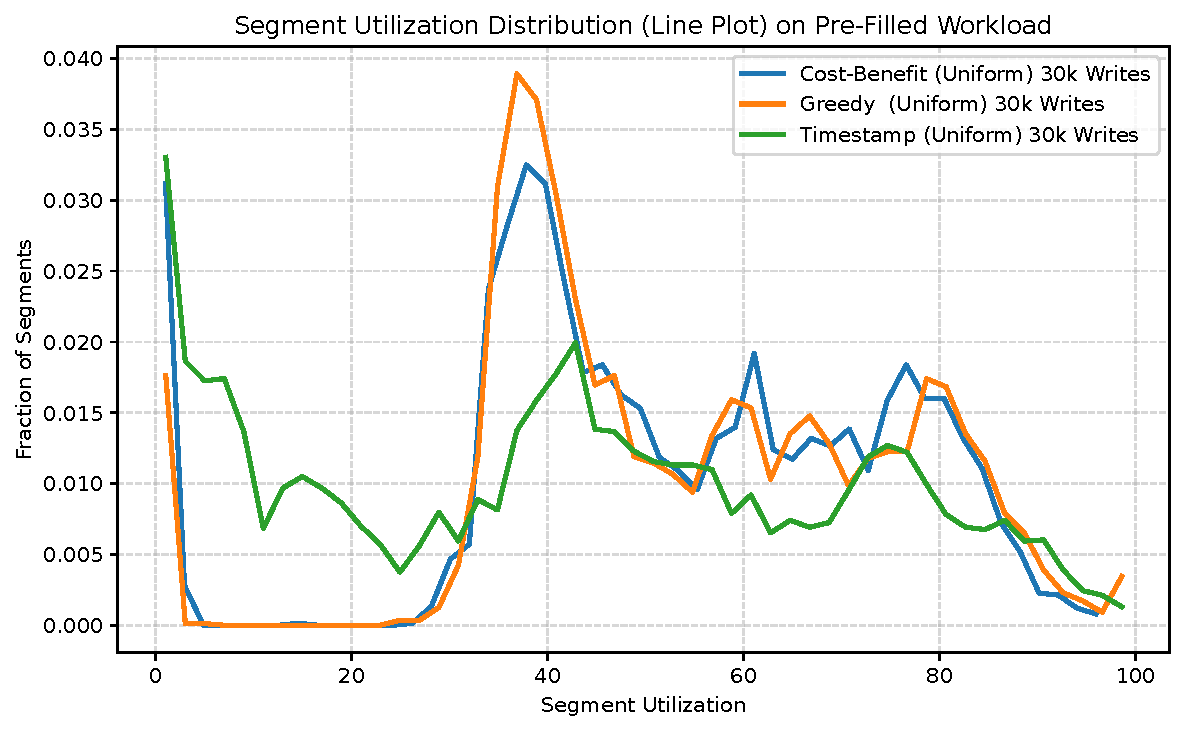
\includegraphics[width=0.5\textwidth]{nilfs_seg_images/all_uniform.pdf}
    \captionof{figure}{Segment utilization distribution for uniform 30k write workload under three policies.}
    \label{fig:all_uniform}
\end{figure}

According to Figure \ref{fig:all_uniform}, cost-benefit, greedy, and timestamp perform approximately the same for segment utilization across uniform writes. Timestamp is a good approximation of cost-benefit or greedy as a segment's utilization falls evenly with age. In the graph of only 30k writes, timestamp performs a marginally worse than greedy and cost benefit. This is largely due to variance and as writes continue, utilization largely converges for all three policies on the uniformly random workload. \\

\subsection{Non-Uniform Segment Utilization}

\subsubsection{Workloads}
We propose two workloads with hot and cold segments with the assumption that many realistic workloads share a similar write pattern of some files that are updated very frequently and others that are updated much less frequently, particularly databases whose journals and data pages may be written very frequently but whose index pages are written far less often. \\

Figure \ref{fig:cb_write_seg} shows an interesting trend: as the number of writes increases from 30k to 1500k, cold segments emerge and retain their utilization, creating a natural segregation between hot and cold segments. \\

\begin{figure}[h] % "h" means place it approximately here
    \centering
    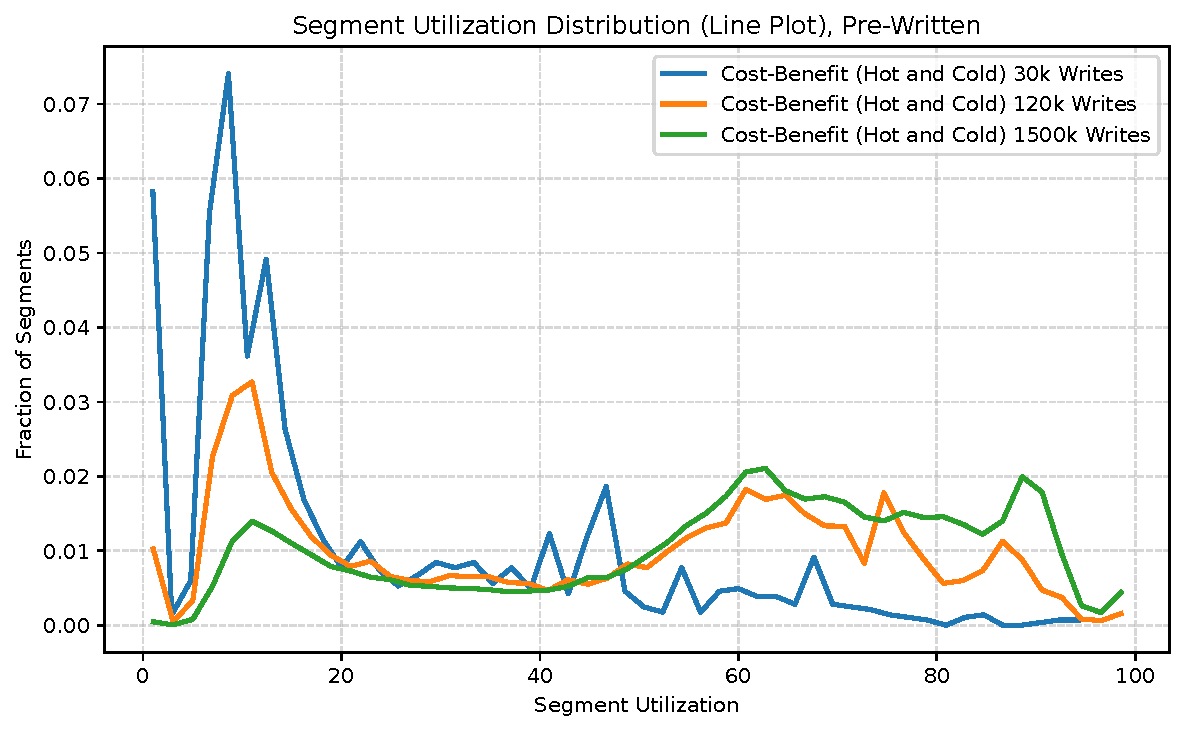
\includegraphics[width=0.5\textwidth]{nilfs_seg_images/cb_write_seg.pdf}
    \captionof{figure}{Segment utilization distribution for hot–cold workload under increasing write counts.}
    \label{fig:cb_write_seg}
\end{figure}

We hypothesize that cost-benefit requires a spatial or temporal buffer to segregate hot and cold segments. Using a pre-written workload can offset this buffer by manually performing segregation. Figure \ref{fig:cb_prefill} confirms this hypothesis, showing a similar split in the pre-written workload with a much higher overall utilization. The cleaner is experiences a lower load with the already settled space and can be much more aggressive on older cold segments. This happens as an artifact of our workload. Initial segments are filled with all hot files or all cold files; therefore, as the program runs, the segments continue to stay segregated by temperature. \\

\subsubsection{Comparison of Policies}

\begin{center}

% Row 2 ----------------------------------------------------
\begin{minipage}{0.45\linewidth}
    \centering
    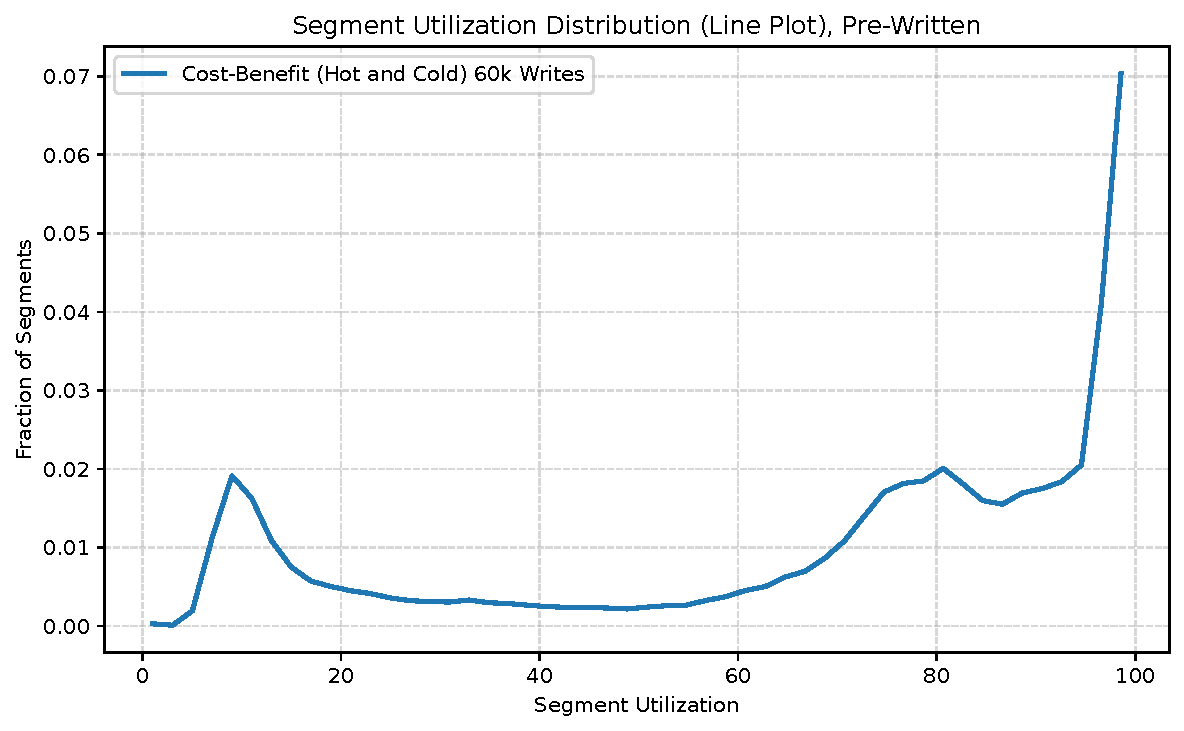
\includegraphics[width=\linewidth]{nilfs_seg_images/cb_prefill.pdf}
    \captionof{figure}{Hot–cold workload with pre-filled segments. (Note that the spike at 100\% segment utilization is expected since our workload plots all dirty segments whereas Sprite LFS plots only segments available for cleaning. This means many segments are fully utilized which is good. )}
    \label{fig:cb_prefill}
\end{minipage}
\hfill
\begin{minipage}{0.45\linewidth}
    \centering
    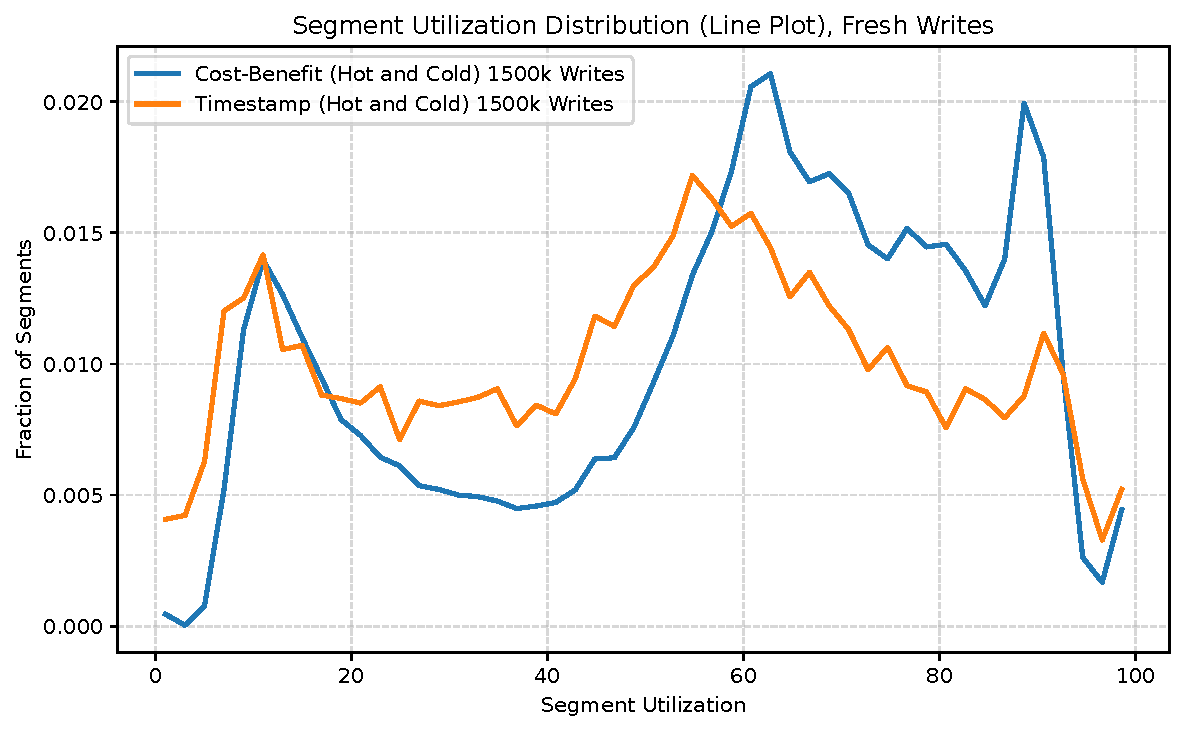
\includegraphics[width=\linewidth]{nilfs_seg_images/hc_t-cb.pdf}
    \captionof{figure}{Timestamp vs Cost–Benefit (1500k writes). We no longer see the spike at 100\% segment utilization compared to the pre-filled workload since the pre-filled workload fills segments so that they can stay at 100\% utilization for a while. }
    \label{fig:hc_t-cb}
\end{minipage}

\vspace{1em}
\end{center}

Figure \ref{fig:hc_t-cb} shows that cost-benefit performs better than timestamp under non-uniform write access. Timestamp over prioritizes cold segments and rewrites them more frequently than cost-benefit. This leads to wasted effort on cold segments that do not need to be refreshed yielding lower segment utilization overall for timestamp.  \\

Likewise, Figure \ref{fig:hc_g-cb} shows that cost-benefit performs better than greedy as well. Greedy over-cleans hot segments and under-cleans cold segments, resulting in a large amount of utilization at 60\%. This also translates to better write costs for cost-benefit as shown in Section 4.3. \\

\begin{center}

% Row 3 ----------------------------------------------------
\begin{minipage}{0.45\linewidth}
    \centering
    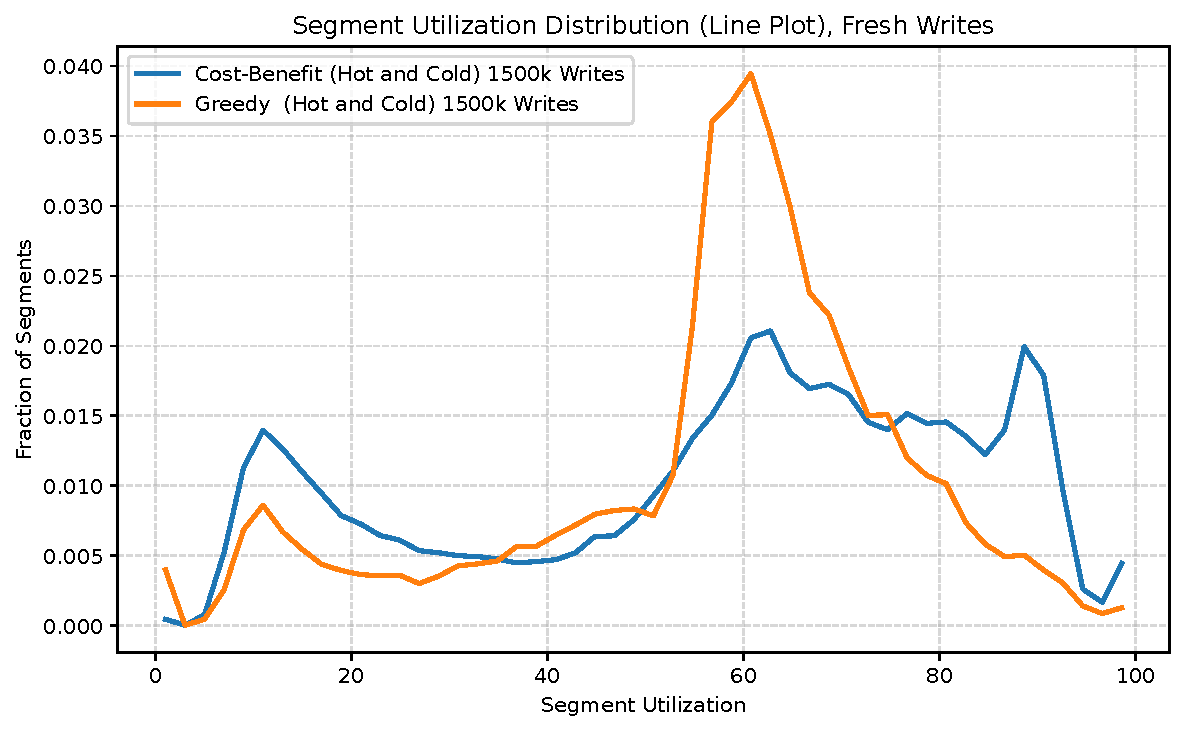
\includegraphics[width=\linewidth]{nilfs_seg_images/hc_g-cb.pdf}
    \captionof{figure}{Greedy vs Cost–Benefit (1500k writes).}
    \label{fig:hc_g-cb}
\end{minipage}
\hfill
\begin{minipage}{0.45\linewidth}
    \centering
    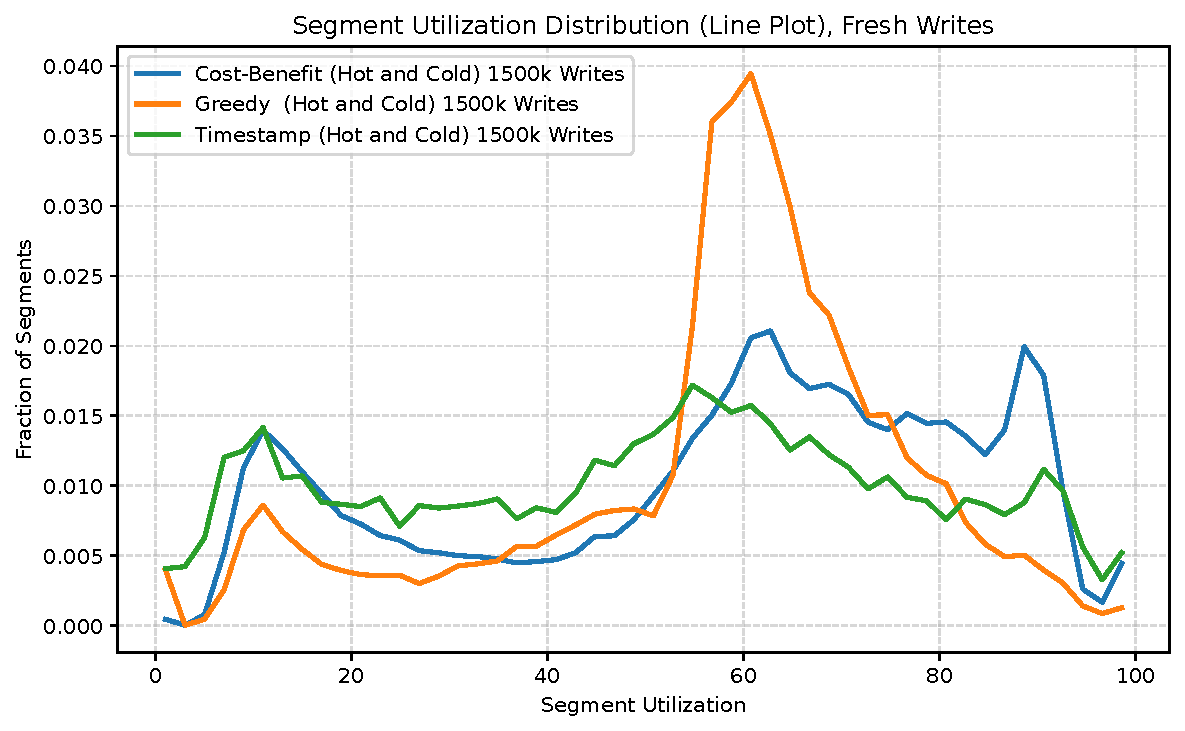
\includegraphics[width=\linewidth]{nilfs_seg_images/hc_t-g-cb.pdf}
    \captionof{figure}{Timestamp vs Greedy vs Cost–Benefit (1500k writes).}
    \label{fig:hc_t-g-cb}
\end{minipage}

\end{center}
\subsubsection{Proactive Segregation}

\begin{figure}[H] % "h" means place it approximately here
    \centering
    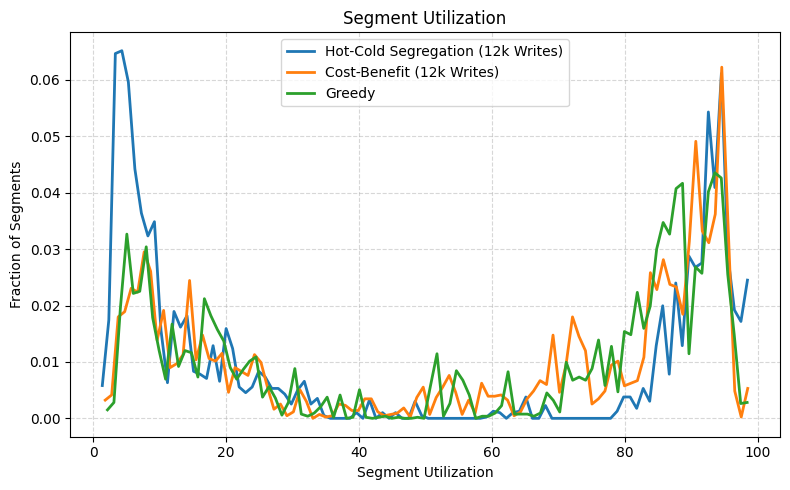
\includegraphics[width=0.5\textwidth]{nilfs_seg_images/cold-start-hnc-segregation.png}
    \captionof{figure}{Segment utilization distribution for non-uniform 12k cold start write workload under three policies.}
    \label{fig:cold-start}
\end{figure}

The pre-written workload shows the need for active segregation of hot and cold segments when starting from a cold file system. This is also in systems with highly dynamic working sets since there is not enough time to wait for segments to naturally be segregated. To resolve this, we created an active segregation segment cleaner. We ran a non-uniform access workload for a short period of time (12k writes). Figure \ref{fig:cold-start} shows that cost benefit and greedy perform around the same in a cold start system while the segregation policy develops a bimodal cleaning policy that maximizes cost benefit. 

However, the segregation policy should not be used as the main policy, since it can only clean hot or cold segments at once. This is ideal in a cold-start situation where cost benefit would perform worse with mixed segments, but would suffer in a situation where the cost benefit scores of a hot and cold segment are around the same.

Instead, segregation should be performed where a lot of mixed segments exist. 

\subsection{Non-Uniform Write Cost}
Sprite LFS [Rosenblum et al.] performs batch segment cleaning when the number of clean segments fall below a threshold until the number of clean segments passes a threshold.

We aim to replicate the write cost results of Sprite LFS. Our evaluation workload set a constant initial disk capacity and performs writes using pre-written hot/cold access until all segments are filled. The workload invokes the cleaner daemon manually and cleans until the number of segments passes a threshold proportional to the size of the initial disk capacity. On every clean, the cleaner reports the average write cost $c = \frac{2}{1-u}$. 

\begin{figure}[H] % "h" means place it approximately here
    \centering
    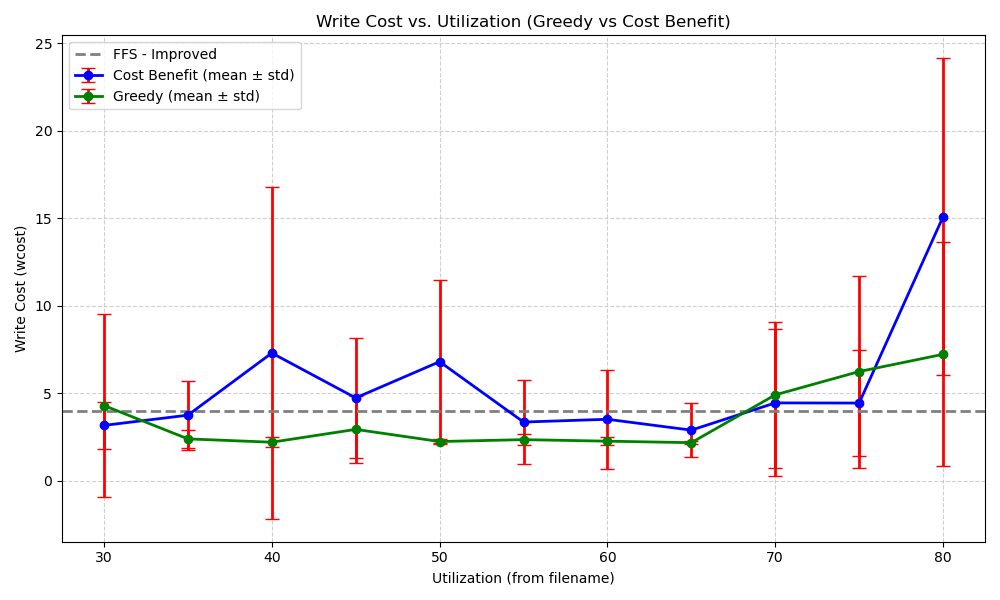
\includegraphics[width=0.5\textwidth]{nilfs_seg_images/write_cost_vs_utilization_comparison.png} % scale image to half the text width
    \caption{Write Cost of Greedy and Cost Benefit (NILFS2) on a hot and cold workflow that gradually fills up the entire disk. }
    \label{fig:wc1}
\end{figure}

Because timestamp and greedy are approximately the same policy within the frame of hot/cold access, we only evaluated the write cost of greedy and cost-benefit. In Figure \ref{fig:wc1} NILFS2 write cost increases as utilization surpasses 60\% for both greedy and cost-benefit similar to Sprite LFS. NILFS2 also surpasss FFS at lower-utilization for writes highlighting a primary strength of NILFS2: small writes and small-file creation. However, cost-benefit and greedy perform around the same in terms of write cost. 

Sprite LFS has a segment size of 1 MB while NILFS2 has a default segment size of 8 MB. The larger segment size allows NILFS2 to have more efficient cleaning and less metadata overhead. Unfortunately, a large segment size means that the natural segment segregation of hot/cold blocks required by cost-benefit takes much longer. We ran our workloads on small disks of 512 MB for short periods of time which did not give the segments much space to be segregated. 

\subsubsection{Alternative Workloads for Non-Uniform Write Cost}

From section 4.2, we argue that cost-benefit requires either time or space to generate accurate results. To see if time plays a factor in write cost, We modified the workload to be temporally scalable. 

\begin{figure}[H] % "h" means place it approximately here
    \centering
    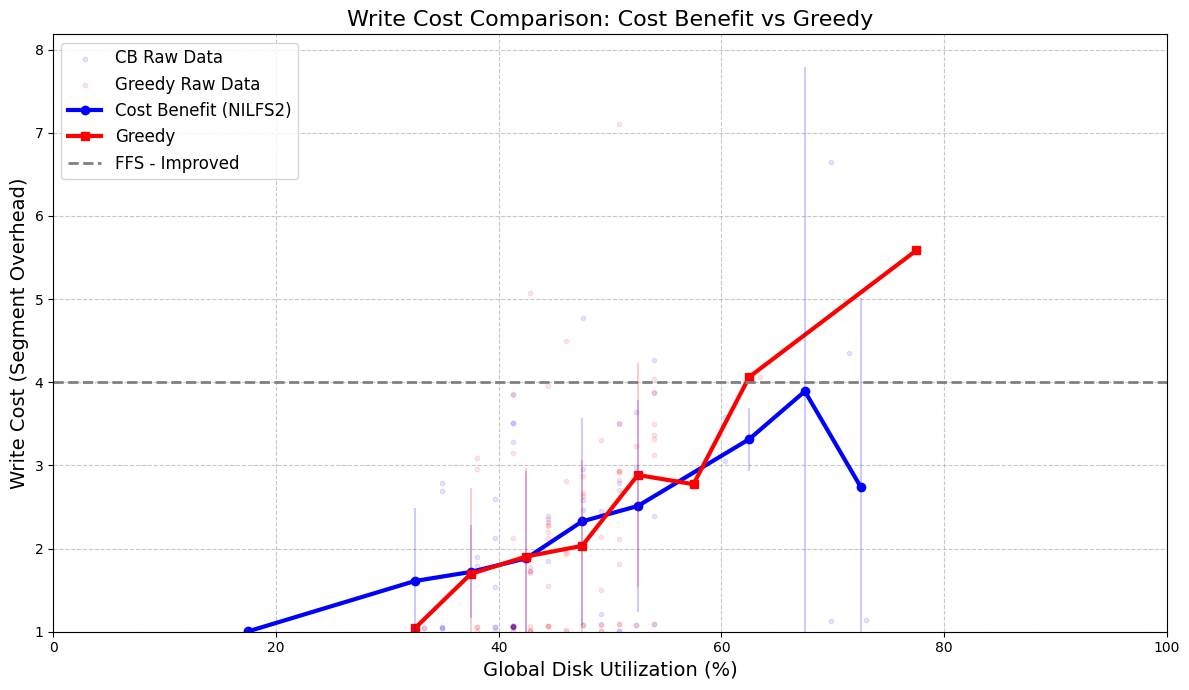
\includegraphics[width=0.5\textwidth]{nilfs_seg_images/wc.png} % scale image to half the text width
    \caption{Write Cost of Greedy and Cost Benefit (NILFS2) on a hot and cold workflow that gradually fills up the entire disk. }
    \label{fig:wc2}
\end{figure}

The modified workload writes repeatedly at a fixed disk capacity using pre-written hot/cold access and runs the cleaner daemon once every 500 writes. The cleaner was modified to clean a maximum of 40 out of 64 available segments. Figure \ref{fig:wc2} indicates that with this workload cost benefit is shown to have a lower write cost than greedy. The  modified workload does not determine write cost with the same precision as the original workload. It instead estimates write cost using: 
\[\frac{1}{m}\sum_{i \in {1..n}} \frac{2}{1-u_i}\]
Where $m = \mathbb{E}[n]$ and $n$ is the number of segments that are actually cleaned. It is actually simple to record $n$ instead of estimating it but due to time constraints, we were unable to modify the cleaner daemon to record $n$ and aggregate the average which would take a significant refactor. 

\section{Conclusion}
\subsection{Future Work}
We propose a modification to the NILFS2 kernel-level implementation in Linux to allow for a hybrid segment cleaner that can dynamically switch between segregation and cost benefit policies. Segregation is ideal when there exist many mixed segments within the system (i.e. segments that may be 90\% cold and 10\% hot but because of the hot-blocks, the age based on last modified time makes the segment appear to the cleaner as a hot segment). Cost benefit is ideal when segments are pre-filled with hot or cold data which is common in many systems. Segregation is necessary since many systems have different working sets for various processes which lead to mixed segments. 

It is computationally expensive and wasteful to track the ages of every block in every segment. We propose to implement a uniform reservoir-sampling algorithm to accurately estimate the "hotness" of a segment. The algorithm is as follows: 

\begin{algorithm}[H]
\caption{NILFS2 Reservoir Write Modification}\label{alg:cap}
\begin{algorithmic}[1]
\State On block-level write to $b$ in segment $s$: 
\State $r_s \gets \{\}, \{u_s, l_s\} \gets \{0, 0\}, K$
\If{$b \in r_s$}
\State update($r_s$, $b$)
\Else
    \If{$l_s < K$}
        \State insert($r_s$, $b$)
        \State $l_s \gets l_s + 1$
    \Else
        \If{rand() $ < K/u_s$}
            \State evict($r_s$, rand() * $K$)
            \State insert($r_s$, $b$)
            \State $u_s \gets u_s+1$
        \EndIf
    \EndIf
\EndIf
\end{algorithmic}
\end{algorithm}

In the algorithm, $r_s$ is the reservoir, a set of at most $K$ blocks and their last modified timestamps. $K$ is a hyperparameter that can be user-tuned. $u_s$ and $l_s$ represent the number of unique writes to blocks (rewrites to the same block do not add to $u_s$) that the reservoir knows about, and the number of elements in the reservoir, respectively. 

As the reservoir represents an accurate sampling of last modified timestamps from blocks in the segment, we can sample the reservoir for an $O(1)$ constant read of the "hotness" of a segment. 


\subsection{Challenges and Mistakes}
We originally set out with a much broader scope of work. One major mistake we made was fixating on replicating the non-uniform bimodal distribution of segment utilization seen when cleaning with cost benefit in Sprite LFS, which took around 40 man hours. Each of our workload runs would take multiple hours (1.5 million+ writes) until we could see the actual bimodal distribution. 

There was a lot of confusion on why the graphs did not match with our hypotheses (and Sprite LFS results). Since there were a lot of contributing factors (i.e. cleaning frequency, watermark thresholds, number of segments cleaned per iteration), it was only with a lot of experimentation and testing that we were able to isolate time as the factor. Instead of fixating on these differences, we should have split up the work more efficiently to create and test more segment cleaning policy ideas. 



\section{Appendix}
\subsection{Specification}
We used a CloudLab EmuLab d430 node for all testing. The filesystem actions were all performed on the SSD on a 20GiB partition. 
\begin{table}[H]
\begin{center}
\resizebox{\columnwidth}{!}{%
\begin{tabular}{c|ccc}
   \Xhline{3\arrayrulewidth}
\hline
\multirow{2}{*}{CPU} & \multicolumn{3}{c}{2 x 2.4 GHz 64-bit 8-Core Xeon E5-2630v3 processor, }\Tstrut\\
& \multicolumn{3}{c}{8.0 GT/s bus speed, 20 MB L3 cache, VT-x ,VT-d, EPT support}\\
\hline
\multirow{2}{*}{Memory} & \multicolumn{3}{c}{8 x 8GB 2133 MT/s DDR4 RAM }\Tstrut\\
& \multicolumn{3}{c}{200 GB 6Gbps SATA SSD, }\Tstrut\\ & \multicolumn{3}{c}{2 x 1 TB 7200 RPM 6 Gbps SATA disks.} \\
\hline
\multirow{1}{*}{OS} & \multicolumn{3}{c}{Ubuntu 22.04.2 LTS}\Tstrut\\
& \multicolumn{3}{c}{Linux kernel 5.15.0}\Tstrut\\
\Xhline{3\arrayrulewidth}
\end{tabular}
}
\caption{Hardware / Software information}
\label{tab:hw-config}
\end{center}
\end{table}
We used nilfs-tools version 2.2.8-1 and forked our dev tools from \href{https://github.com/nilfs-dev/nilfs-utils}{https://github.com/nilfs-dev/nilfs-utils} on commit hash 3e172d19ad654e6f65742b9f81992c656ecc0524.
\subsection{Git}
\href{https://github.com/txst54/nilfs-utils}{https://github.com/txst54/nilfs-utils}

\subsection{Notes}
This project took a total of 70 man-hours. LLMs were used to initially generate boilerplate code for the plugin harness and workload logger in nilfs-utils but we later modified most of the LLM code by hand due to issues (it turns out that LLMs often misinterpret struct field names) or modifications that we wanted to implement. 

\end{document}

